
\documentclass[11pt, aspectratio=169]{beamer}

\usepackage[utf8]{inputenc}
\usepackage{tikz}
\usepackage[english]{babel}
\usepackage{svg}
\usepackage{eurosym}
\usepackage{subfig}
\usepackage{pgfgantt}
\usepackage[export]{adjustbox}
%\usepackage[shortlabels]{enumitem}
\usepackage[font=scriptsize,justification=centering]{caption}

%----------------------------------------------------------------------------------------
%	TITLE PAGE INFORMATION.
%----------------------------------------------------------------------------------------
\author{A. M\"{o}slinger, K. Steele, D. Talavera, N. Ulfvarson, and E.F.M. Weterings}
\title{InfraRed Imaging of astronomical targets with a Stabilised Camera}
\subtitle{IRISC}
\institute{DLR MORABA, Oberpfaffenhofen} 
\date{11-15 February 2019}
%\subject{} 

%----------------------------------------------------------------------------------------
%	SETUP LAYOUT.
%----------------------------------------------------------------------------------------
\usepackage{theme/beamerthemeWarsawLTU}
%\usetheme{Warsaw}


\begin{document}
%----------------------------------------------------------------------------------------
%	TITLE PAGE.
%----------------------------------------------------------------------------------------

{\setbeamertemplate{logo}{}
\begin{frame}
\titlepage
\begin{tikzpicture}[remember picture,overlay]
    \node[xshift=13cm,yshift=-1.025\textheight,anchor=north west] at (current page.north west){%
    
\includegraphics[width=2cm]{theme/LTU_logo.jpg}};
\end{tikzpicture}
\end{frame}
}

%----------------------------------------------------------------------------------------
%	TABLE OF CONTENTS.
%----------------------------------------------------------------------------------------
\begin{frame}[t]{Table of Contents}
\vspace{-0.3cm}
    \begin{columns}[t]
        \begin{column}{.5\textwidth}
            \tableofcontents[sections={1-2}]
        \end{column}
        \begin{column}{.5\textwidth}
            \tableofcontents[sections={3-5}]
            \vspace{-.2cm}
            \tableofcontents[sections=6,hidesubsections]
        \end{column}
    \end{columns}
\end{frame}


%----------------------------------------------------------------------------------------
%	INTRODUCTION. 				% DIEGO
%----------------------------------------------------------------------------------------
\section{IRISC: In a Nutshell}
\begin{frame}[c]{In a Nutshell}
    \centering
    \huge Our vision is to make astronomical research more accessible by developing a stabilised balloon-borne telescope
\end{frame}


%----------------------------------------------------------------------------------------
%	SYSTEM.
%----------------------------------------------------------------------------------------
\section{System}
\subsection{Construction}	 	% DIEGO

\begin{frame}{Construction}
\begin{columns}
	\begin{column}{0.6\textwidth}
%		\hspace{1cm}
		\begin{tabular}{l|r|r}
		Color & Component & Mass \\ \hline
		Yellow & Telescope & 3.66 \, kg \\ 
		Red & NIR Camera & 120 \, g \\ 
		Purple & Gimbal & $<$ 5\, kg\\
		Green & Guiding Camera & $<$ 150 \,g \\
		Blue & Electronics box  & $<$ 2 \,kg
	\end{tabular}
	\end{column}
	\begin{column}{0.4\textwidth}
	\begin{figure}
	\hspace{-3cm}
	\centering
	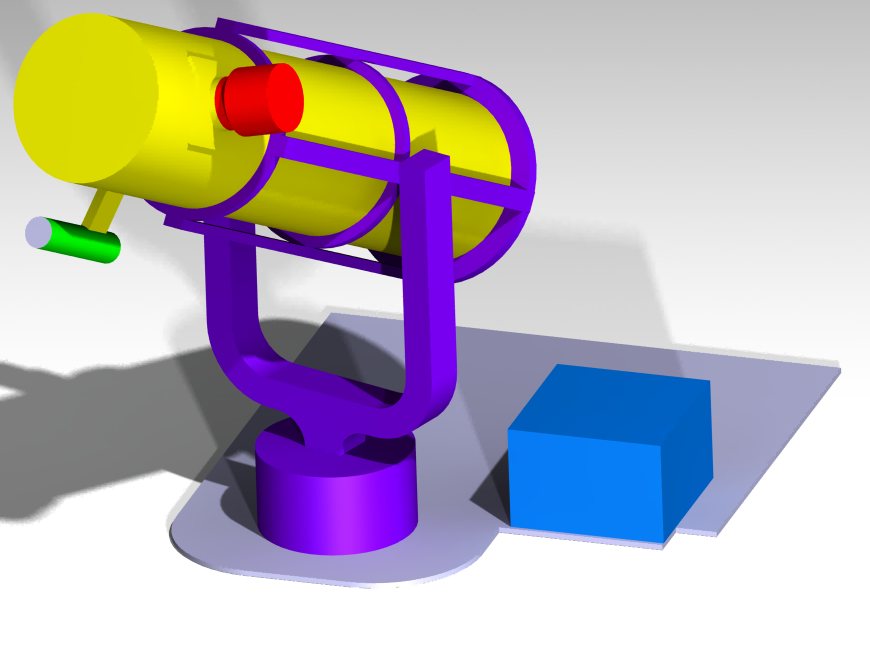
\includegraphics[scale=0.8]{figures/CAD/Outside_Gondola/Experiment.png}
	\end{figure}
	\end{column}
\end{columns}
\end{frame}
\begin{frame}{Construction}
\vspace{-2cm}
\begin{columns}[t]
	\begin{column}{0.4\textwidth}
		\begin{figure}
		\centering		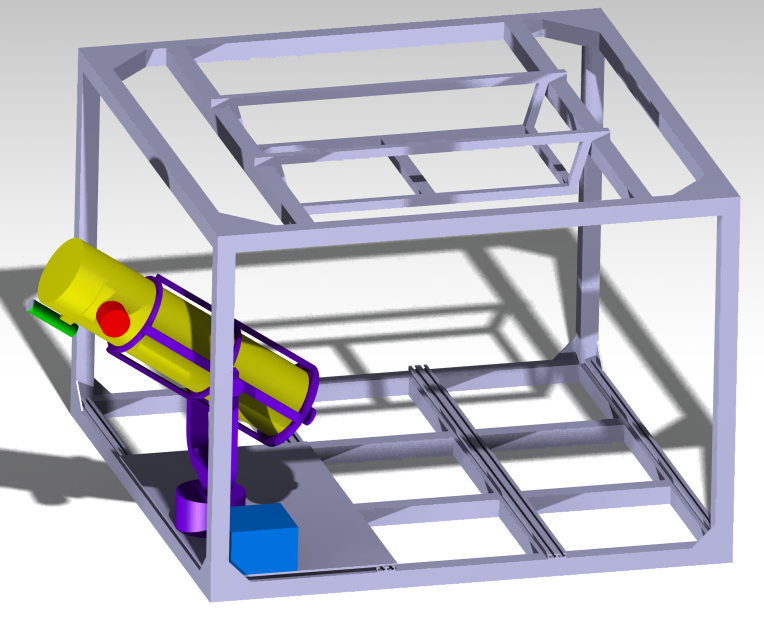
\includegraphics[scale=0.9]{figures/CAD/Inside_Gondola/Iso1.png}
		\end{figure}
	\end{column}
	
	\begin{column}{0.4\textwidth}
		\begin{figure}
		\centering
		\vspace{0.5cm}
	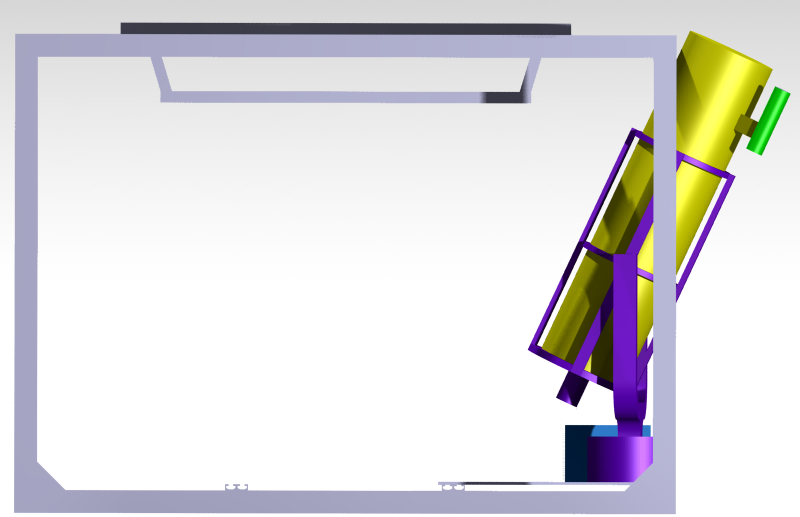
\includegraphics[scale=0.9]{figures/CAD/Inside_Gondola/Vertical_lim.png}
		\end{figure}
	\end{column}
\end{columns}
%Updated CAD design with the correct location and size. Would be a huge plus if it can rotate a bit.
\end{frame}

\begin{frame}{Contruction}
\vspace{-1cm}
\begin{columns}[t]
	\begin{column}{0.4\textwidth}
		\begin{figure}
		\centering		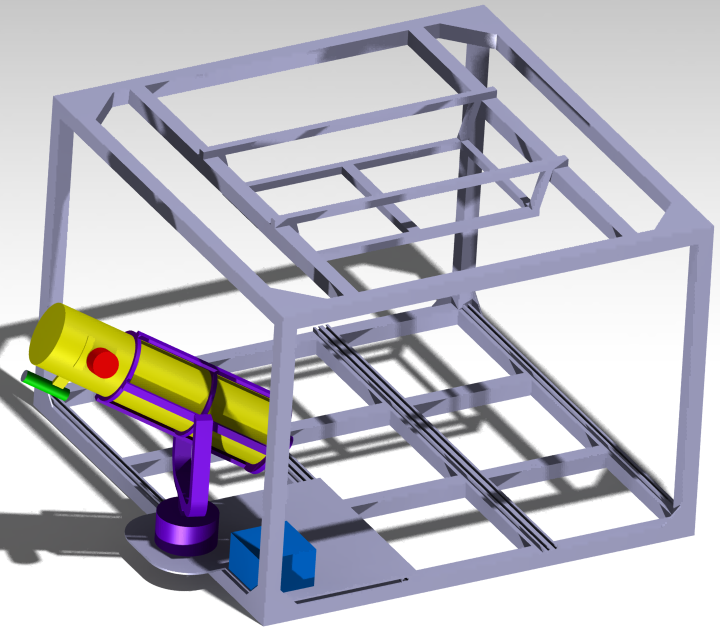
\includegraphics[scale=0.9]{figures/CAD/Outside_Gondola/Iso2.png}
		\end{figure}
	\end{column}
	
	\begin{column}{0.4\textwidth}
		\begin{figure}
		\centering
%		\vspace{-1cm}
	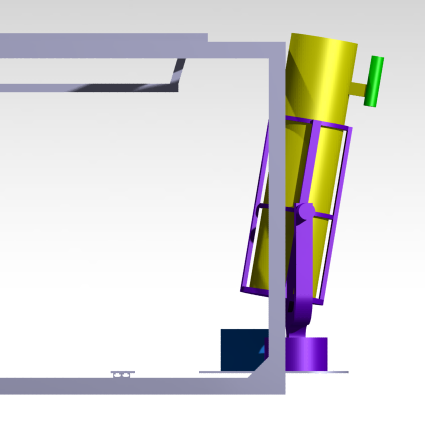
\includegraphics[scale=1.3]{figures/CAD/Outside_Gondola/Vertical_lim.png}
		\end{figure}
	\end{column}
\end{columns}
\end{frame}

\subsection{Thermal} 			% DIEGO
\begin{frame}{Thermal}
\begin{itemize}
	\item Telescope structure will act as a baffle
	\item FEA will be used to determine cooling or heating requirements for electronic components
	\item Heating pads will be used to prevent the motors from freezing
	\item NIR camera will be cooled to ensure performance
\end{itemize}

\end{frame}

\subsection{Electrical Setup}	% ELRICK
\begin{frame}[c]{Electrical ACD}
\centering
\begin{figure}
	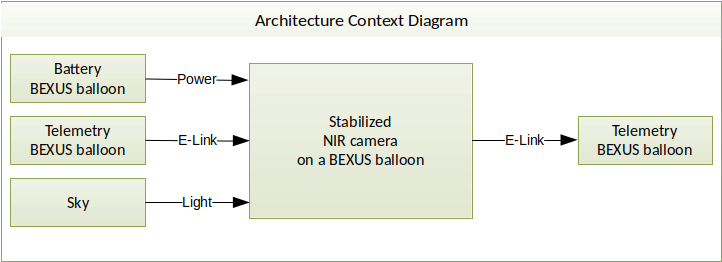
\includegraphics[width=.8\textwidth]{figures/images/elec_ACD.png}
\end{figure}
\end{frame}

\begin{frame}{Electrical AID}
\begin{figure}
	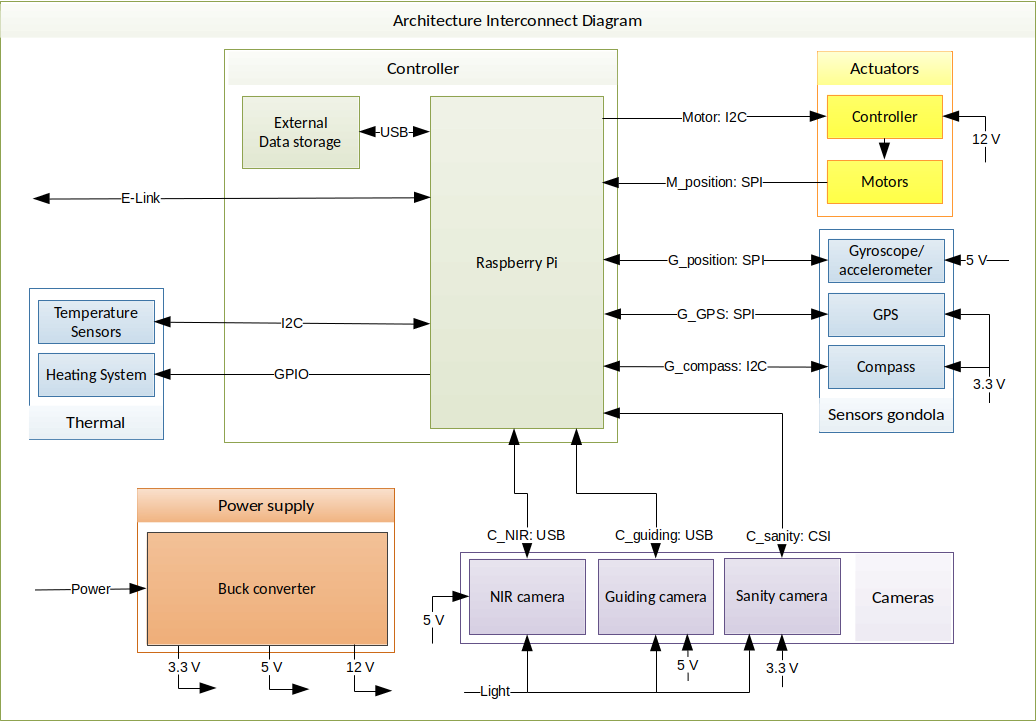
\includegraphics[width=.65\textwidth]{figures/images/elec_AID.png}
\end{figure}
\end{frame}

\begin{frame}{Power Consumption}
\centering
	\begin{tabular}{| l | l | l | l |}
	\hline
	& \textbf{Power [W]} & \textbf{On-time [\%]} & \textbf{Energy 4h [Wh]} \\\hline\hline
	NIR camera 		& 1.5	 	& 100 & 6 		\\\hline
	Guiding camera 	& 1.5 		& 100 & 6		\\\hline
	Controller 		& 6.25 		& 100 & 25		\\\hline
	Sensors 		& 1			& 100 & 4		\\\hline
	Motors			& 3 x 4.2	& 100 & 50.4	\\\hline
	Heating system 	& 10		& 20  & 8		\\\hline\hline
	
	\textbf{Subtotal:}& & 			  & 99.4 Wh \\\hline\hline
	
	Standby P (6h) 	& & 			  & 40 Wh	\\\hline\hline
	
	\textbf{Total:} & & 			  & 139.4 Wh\\\hline
	\end{tabular}
\end{frame}

\begin{frame}[c]{Onboard Storage}
\centering
\hspace*{-.5cm}
\begin{tabular}{| l | l | l | l | l |}
	\hline
	\textbf{Item} & \textbf{File size} & \textbf{Compressed file size} & \textbf{Sample rate} & \textbf{Total storage (3h)} \\\hline\hline
	
	NIR camera		& 30\,MB  & 18\,MB & 60\,sec 	 & 5.5\,GB \\\hline
	Guiding camera	& 3.5\,MB & 2\,MB  & 15\,sec	 & 2.5\,GB \\\hline
	Sanity camera	& 8\,MB   & 5\,MB  & On request  & - \\\hline
	Sensors			& 75\,B   & -      & 0.1-1\,sec  & 8.1-0.81\,MB \\\hline\hline
	\textbf{Total:} &	   	  &	       &	         & 8\,GB \\\hline
	

\end{tabular}
\end{frame}

\begin{frame}[c]{Downlink Bandwidth}
\centering
\hspace*{-.3cm}
\begin{tabular}{| l | l | l | l |}
	\hline
	\textbf{Item} & \textbf{File size} & \textbf{Downlink rate} & \textbf{Datarate} \\\hline\hline
	
	NIR camera (20 pictures ) & 18\,MB & 60\,sec & 0.55\,Mbits/sec (over 90 min) \\\hline
	Guiding camera		   & 2\,MB	& 60\,sec	& 0.28\,Mbits/sec \\\hline
	Sanity camera		   & 5\,MB  & On request& - \\\hline
	Sensors				   & 30\,B  & 1\,sec 	& 240\,bits/sec \\\hline\hline
	\textbf{Total:} 	   &		& 			& 0.83\,Mbits/sec \\\hline
	

\end{tabular}
\end{frame}

\subsection{Ground Station} 	% NIKLAS
\begin{frame}{Ground Station}
\begin{itemize}
	\item K.I.S.S.
	\item Written in C with GTK+
	\item \texttt{reset, target, stowage}
\end{itemize}
\begin{figure}
	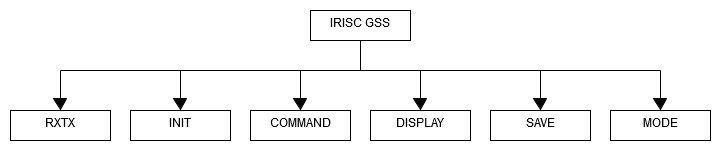
\includegraphics[scale=0.4]{figures/images/GSS-tree.png}
\end{figure}
\end{frame}

\subsection{On-board Software} 	% NIKLAS
\begin{frame}{On-board Software}
\begin{itemize}
	\item The glue between the systems
	\item C on a simple linux distro
	\item Compression and storage
\end{itemize}
\begin{figure}
	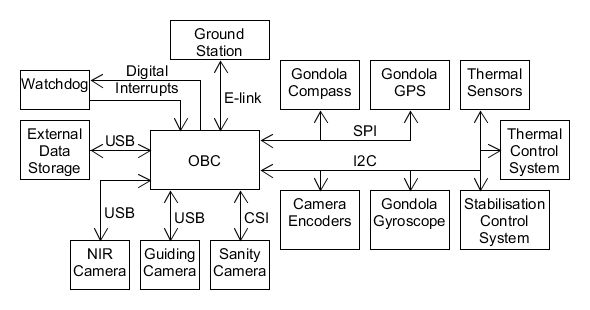
\includegraphics[scale=0.4]{figures/images/process-overview.png}
\end{figure}
\end{frame}

\subsection{Control System} 	% ANJA
\begin{frame}[t]{Control system}
\begin{itemize}
	\item<1-> Stabilisation of the gimbal: dynamic control system (e.\,g.~PID) %\\
	\begin{itemize}
		\item Mechanical model of the gimbal, motors model
		\item Sensor data: gyroscopes, accelerometer%\\
	\end{itemize}
%		Sensor data: gyroscopes, accelerometer%\\
%		Includes mechanical model of gimbal, motors
	\item<2-> Selection of targets: %\\
	\begin{itemize}
		\item Based on prioritisation parameters (e.\,g. brightness, location)
		\item Sensor data: magnetometer, GPS, gyroscopes, encoders %\\
	\end{itemize}
%		Sensor data: magnetometer, GPS, gyroscopes, encoders %\\
%		Includes model of movements of astronomical targets
	\item<3-> Tracking of targets: 
	\begin{itemize}
		\item Model of movements of astronomical targets
		\item Sensor data: gyroscopes, encoders
	\end{itemize}
	\item<4-> Feedback loop, measured states: 
	\begin{itemize}
		\item Kalman filter determines exact position \& orientation
	\end{itemize}
	%utilisation of a Kalman filter to determine exact position \& orientation
\end{itemize}

\end{frame}

\begin{frame}[t]{Control system}
Minor objectives of the control system:
\begin{itemize}
	\item Avoid looking directly into the Sun
	\item Thermal control of the camera sensor and electronics
	\item Motor control
\end{itemize}

\end{frame}

\subsection{Cameras} 			% ANJA
\begin{frame}{NIR Camera for the telescope}
\vspace{-0.2cm}
\begin{columns}[t]
\begin{column}{0.6\textwidth}
	\begin{itemize}
		\item CMOS Sensor: ZWO ASI183MM (mono-colour) \\
			resolution: 20.18\,MP, sensor size: 13.2x8.8\,mm
		\item NIR-conversion with 720\,nm NIR filter
		%\item Sensitivity: 720\,nm to 1150\,nm
		\item Rolling shutter: no mechanical shutter, no moving parts
	\end{itemize}
	\vspace{-0.7cm}
	\begin{figure}
	\centering
	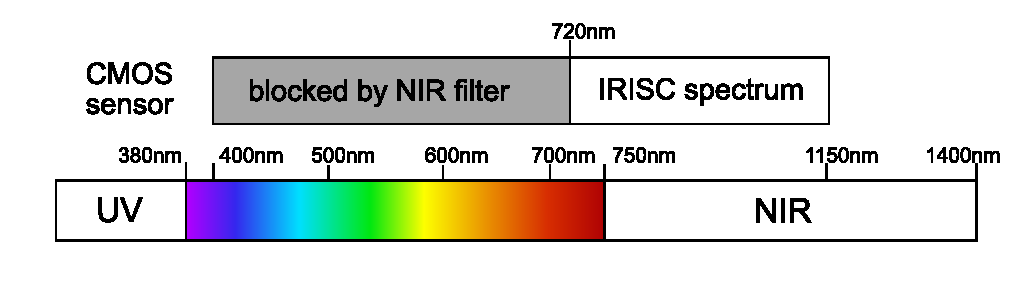
\includegraphics[width = 1.1\linewidth]{figures/images/IRISC_spectrum.eps}
\end{figure}
\end{column}
\begin{column}{0.4\textwidth}
	\begin{figure}[t]
		\centering
		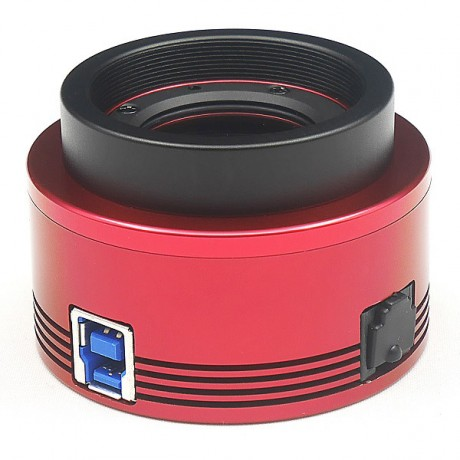
\includegraphics[width=0.7\linewidth]{figures/images/ZWO_ASI183MM.jpg}
		\caption*{Credits: ZWO ASI183MM (mono)}
		\label{fig::NIR_sensor}
	\end{figure}
\end{column}
\end{columns}
\end{frame}

\begin{frame}{Guiding Camera}
\begin{columns}[t]
\begin{column}{0.6\textwidth}
\begin{itemize}
	\item For verification of the field of view (7.5\,deg)
	\item Support of ground-based re-calibration of sensors (e.\,g.~magnetometer, gyroscopes)
	\item Imaging sensor with a high sensitivity, resulting in shorter exposure times (compared to NIR camera)
	\item Imaging in visible wavelengths and NIR
\end{itemize}

\end{column}
\begin{column}{0.4\textwidth}
	\begin{figure}[t]
		\centering
		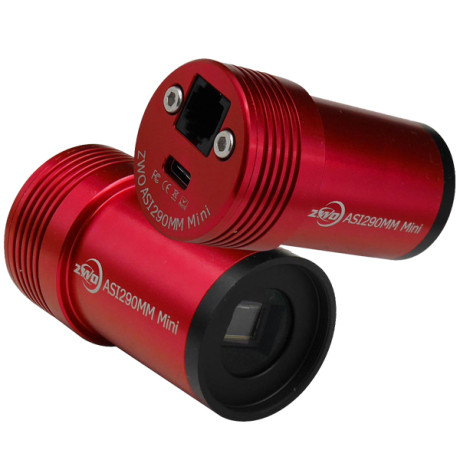
\includegraphics[width=0.7\linewidth]{figures/images/ZWO_ASI290MM_Mini.jpg}
		\caption*{Credits: Guiding camera by ZWO}
		\label{fig::guiding_camera}
	\end{figure}
\end{column}
\end{columns}
\end{frame}

%\begin{frame}{Sanity Camera}
%probably not going to be included in the presentation - any objections?
%\end{frame}

\subsection{Telescope} 			% KIM
\begin{frame}{Telescope}
\begin{figure}[!htb]
    \centering
    \begin{minipage}{.5\textwidth}
        \centering
        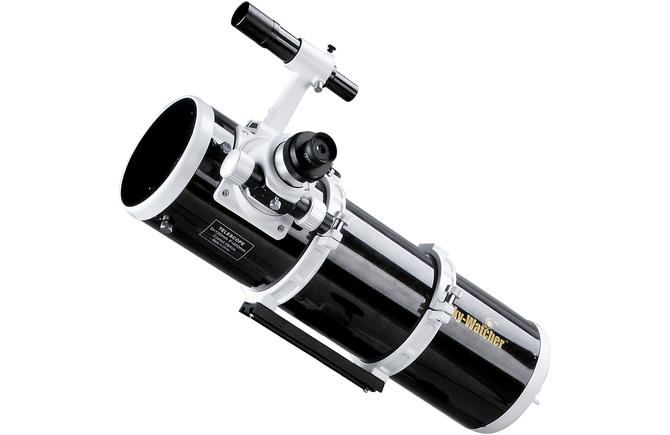
\includegraphics[width=\linewidth]{figures/images/SkyWatcher_BKP130DS.jpg}
        \caption*{SkyWatcher BKP 130DS (with eyepiece in place of the camera)}
    \end{minipage}%
    \begin{minipage}{0.5\textwidth}
    SkyWatcher BKP 130DS
    \begin{itemize}%[label=--]
        \item Newtonian telescope 
        \item Focal length: 650\,mm 
        \item Aperture: 130\,mm
        \item FOV: 1.16\,deg by 0.78\,deg 
        \item Diffraction-limited-resolution: 1.94\,arcsec
        \item Pixel size: 0.76\,arcsec (in \newline combination with the camera)
    \end{itemize}
    \end{minipage}
\end{figure}
\end{frame}


%----------------------------------------------------------------------------------------
%	SCIENCE. 					  KIM
%----------------------------------------------------------------------------------------
\section{Science}
\subsection{Targets}
\begin{frame}{Targets}
\vspace{-0.27cm}
\begin{figure}[!htb]
    \begin{minipage}[t]{.425\textwidth}
        \centering
        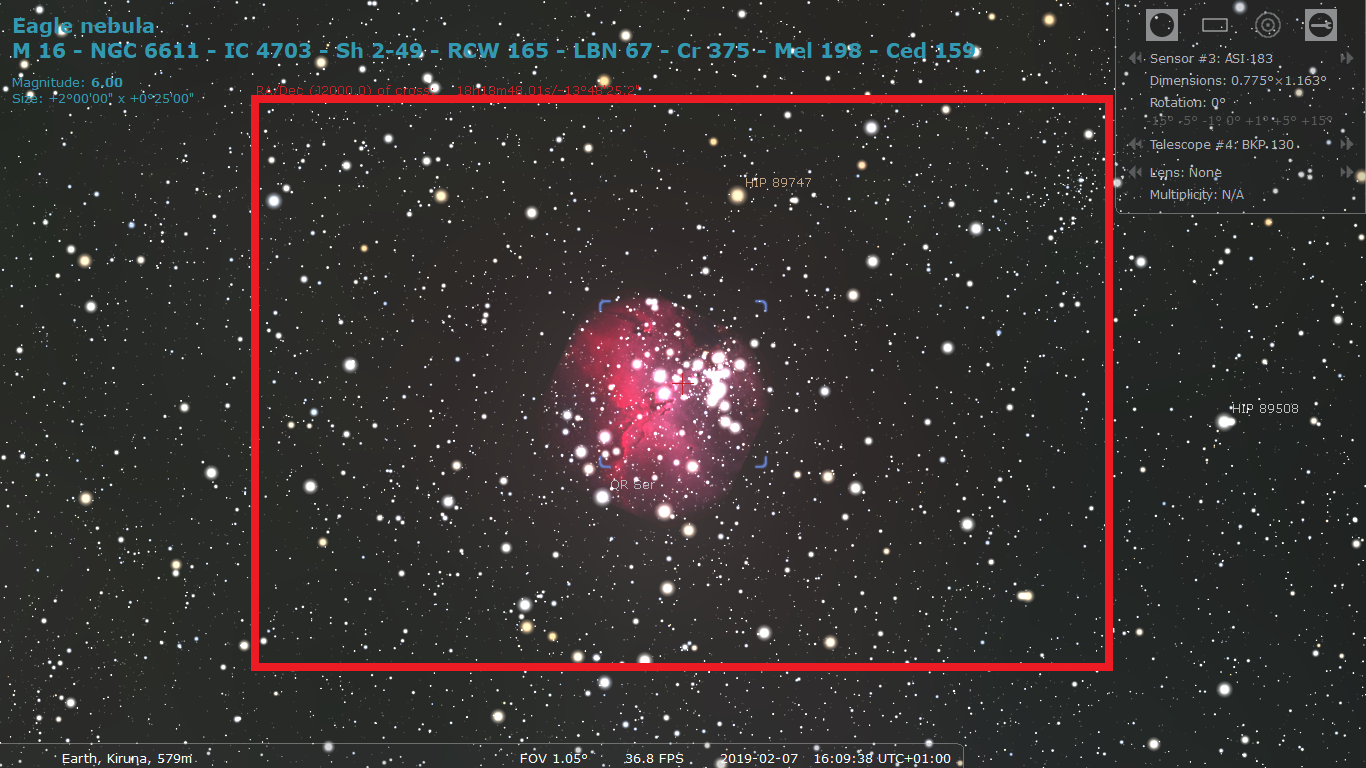
\includegraphics[width=\linewidth]{figures/targets/Eagle.png}
    \end{minipage}%
	\begin{minipage}[t]{.425\textwidth}
        \centering
        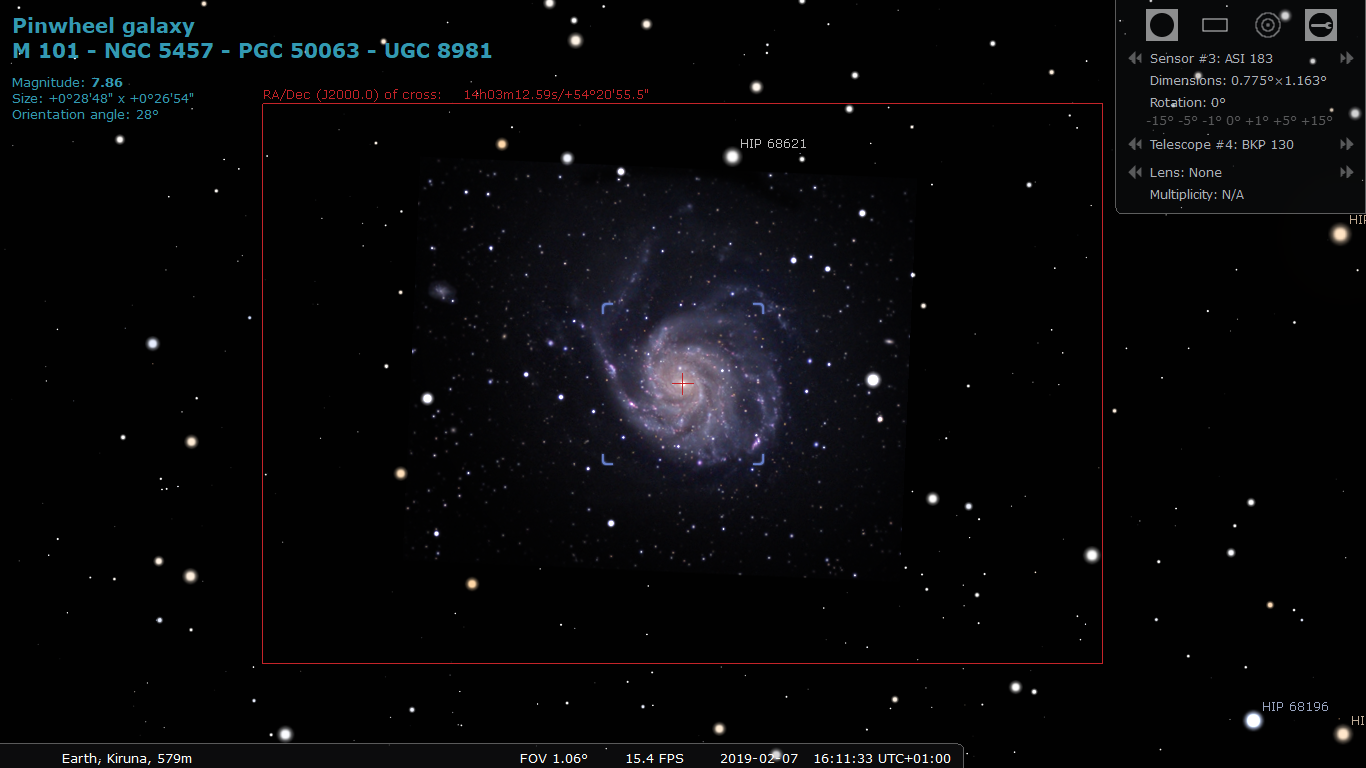
\includegraphics[width=\linewidth]{figures/targets/Pinwheel.png}
    \end{minipage}%
	\vspace{-0.02cm}  
    \begin{minipage}[t]{.425\textwidth}
        \centering
        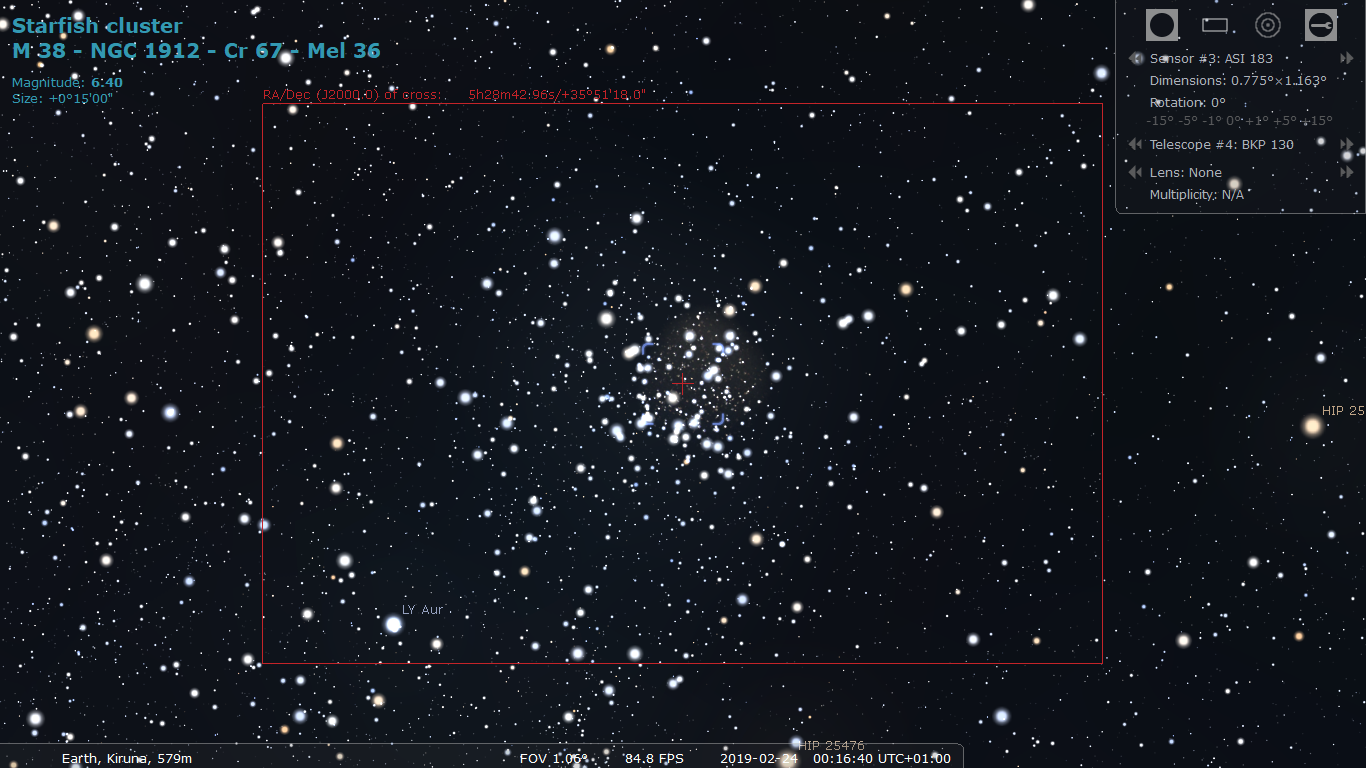
\includegraphics[width=\linewidth]{figures/targets/Starfish.png}
    \end{minipage}%
    \begin{minipage}[t]{.425\textwidth}
        \centering
        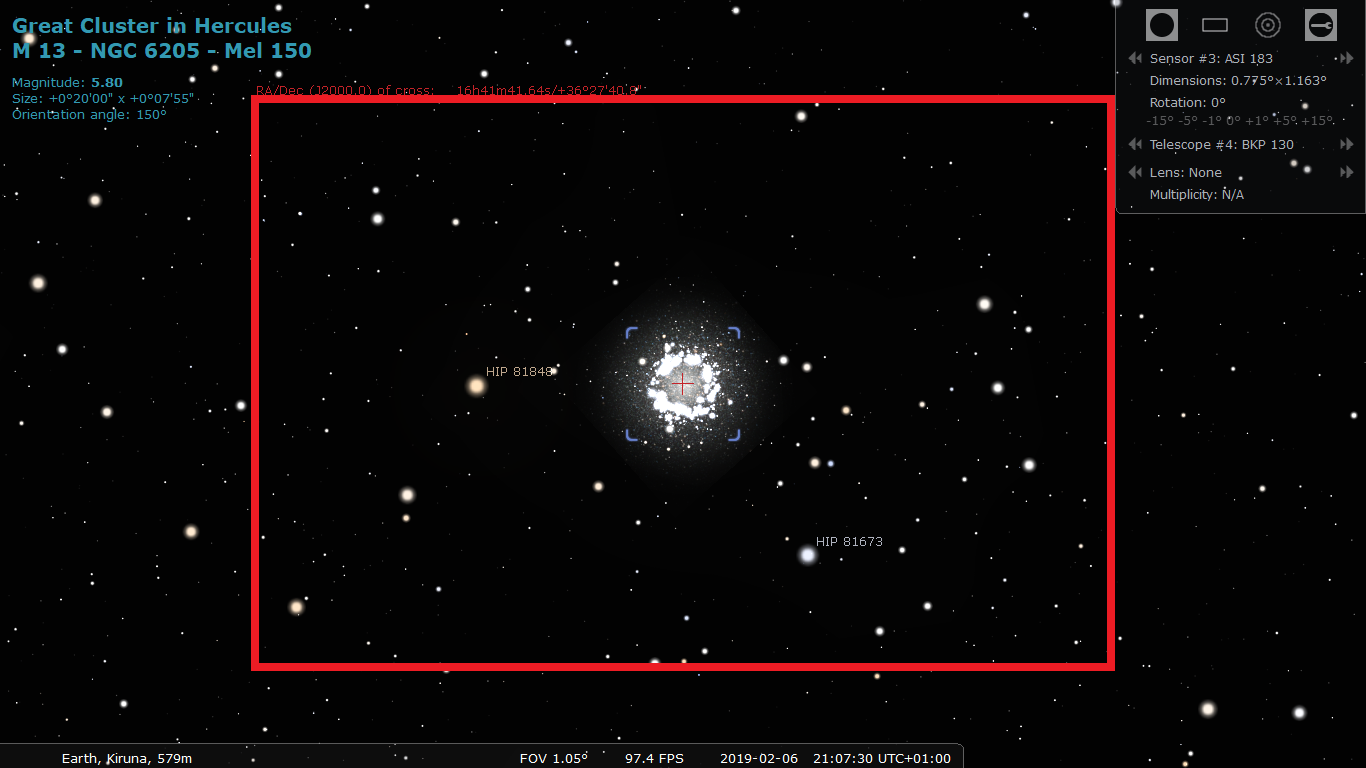
\includegraphics[width=\linewidth]{figures/targets/Hercules.png}
    \end{minipage}%
\end{figure}
\end{frame}

\subsection{Signal to Noise Ratio}
\begin{frame}{Signal to Noise Ratio}
\begin{figure}[!htb]
    \hspace{-2cm}
    \begin{minipage}{0.6\textwidth}
        \centering
        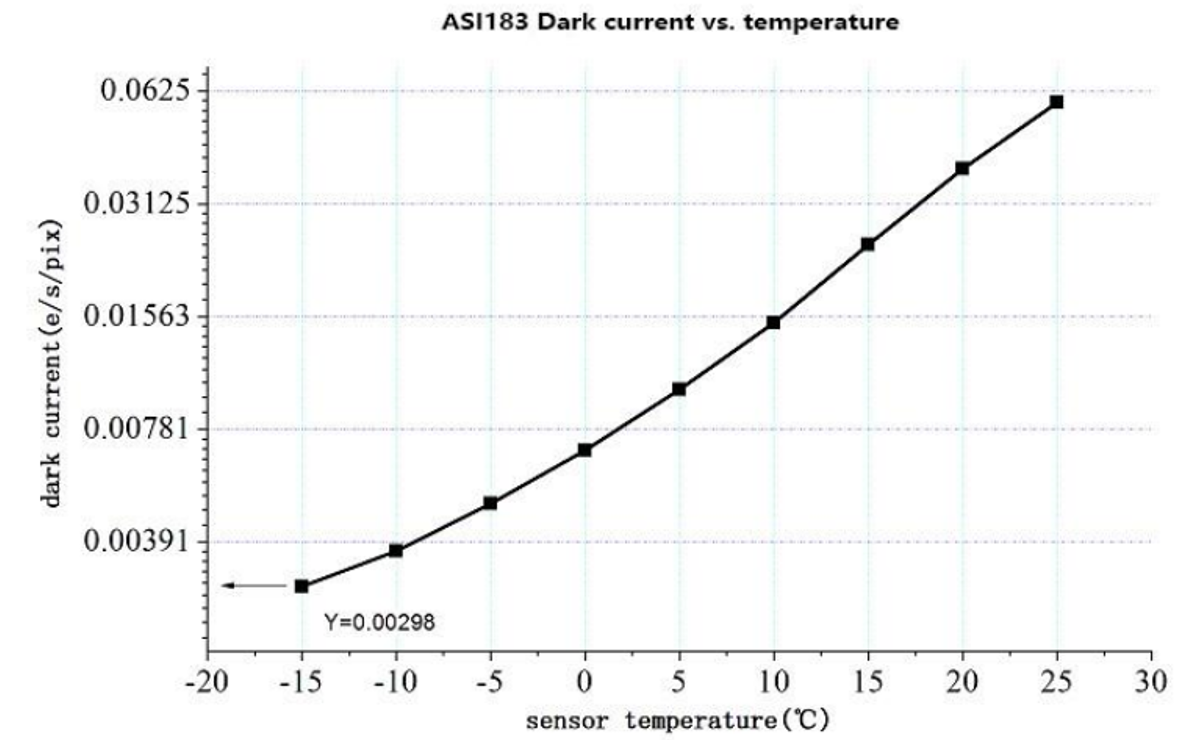
\includegraphics[width=0.9\linewidth]{figures/images/darkcurrent.PNG}
        \caption{Dark current vs. temperature as given in the camera manual}
    \end{minipage}%
    \begin{minipage}{0.2\textwidth}
	 	\centering
	 	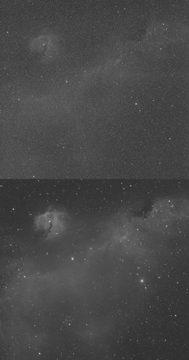
\includegraphics[width=0.9\linewidth]{figures/images/Uncool-189x360.jpg}
	 	\caption*{Credit: Richard S. Wright Jr., SkyandTelescope.com}
    \end{minipage}
\end{figure}
\end{frame}

\subsection{Data Analysis}
\begin{frame}{Data Analysis}
\begin{figure}[!htb]
    \centering
    \hspace{-0.9cm}
    \begin{minipage}{0.65\textwidth}
        \centering
        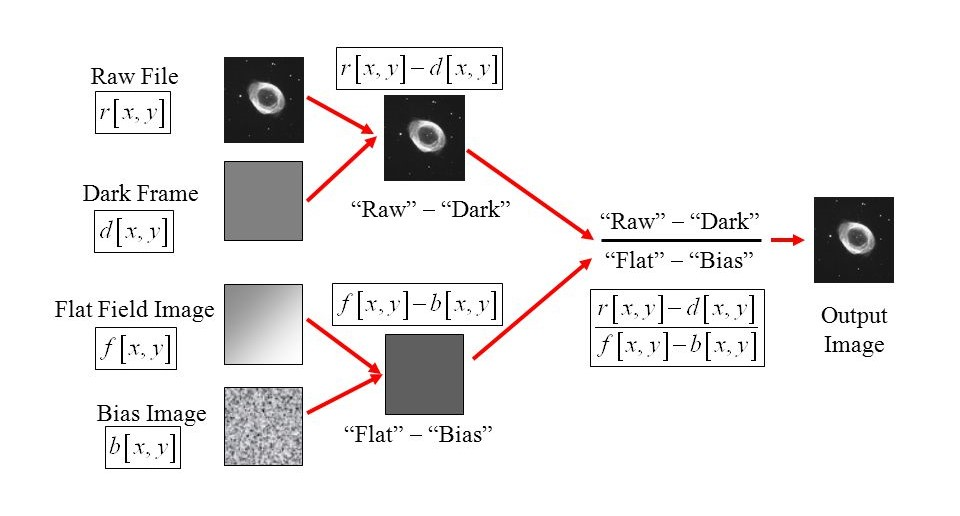
\includegraphics[width=\linewidth]{figures/images/correctionpipeline.jpg}
        \caption{Standard astrophotography image calibration pipeline}
    \end{minipage}%
    \begin{minipage}{0.35\textwidth}
    \begin{itemize}%[label=--]
        \item \textbf{Light Frames:} image of the target itself
        \item \textbf{Dark Frames:} aperture blocked of light
        \item \textbf{Flat Frames:} brightness balance of the sensor
        \item \textbf{Bias Frames:} readout noise due to the sensor
    \end{itemize}
    \end{minipage}
\end{figure}
\end{frame}


%----------------------------------------------------------------------------------------
%	PROJECT MANAGEMENT.
%----------------------------------------------------------------------------------------
\section{Project Management}
\subsection{Schedule}
{\setbeamertemplate{logo}{}
\begin{frame}{Schedule} 		% DIEGO
\begin{ganttchart}[
	hgrid,
	vgrid,
	expand chart=\textwidth,
	time slot format=isodate-yearmonth,
	time slot unit=month,
	y unit chart=.5cm,
	y unit title=.7cm
	]{2018-12}{2020-02}
	\gantttitle{BEXUS - IRISC}{13}\\
	\gantttitlecalendar{year, month=shortname} \\
	\ganttbar{Design Phase}{2018-12}{2019-04}\\
	\ganttbar{Unit testing}{2019-03}{2019-05}\\
	\ganttbar{Manufacturing Phase}{2019-04}{2019-07}\\
	\ganttmilestone {Manufacturing milestones}{2019-04} 
	\ganttmilestone {}{2019-09}\\
	\ganttbar{Complete System Testing}{2019-06}{2019-09}\\
	\ganttbar{Launch Campaign}{2019-10}{2019-10}\\
	\ganttbar{Data Analysis Phase}{2019-11}{2019-12}\\
	\ganttmilestone {Reviews} {2019-01} 
	\ganttmilestone {} {2019-05}
	\ganttmilestone {} {2019-07}
	\ganttmilestone {} {2019-08}
	\ganttmilestone {} {2020-01}
	
\end{ganttchart}

% global & zoomin
\end{frame}}

\subsection{Outreach} 			% NIKLAS
\begin{frame}{Outreach}
\begin{figure}[!htb]
	\centering
    \begin{minipage}{0.5\textwidth}
    \vspace{-2cm}
    Website and social media:
    	\begin{itemize}
    		\item Website - www.irisc.space
    		\item Facebook - @IRISCBexus
    		\item Twitter - @IRISCBEXUS
    		\item Instagram - @Irisc\_bexus
    	\end{itemize}
    \end{minipage}%
    \begin{minipage}{.5\textwidth}
        \centering
        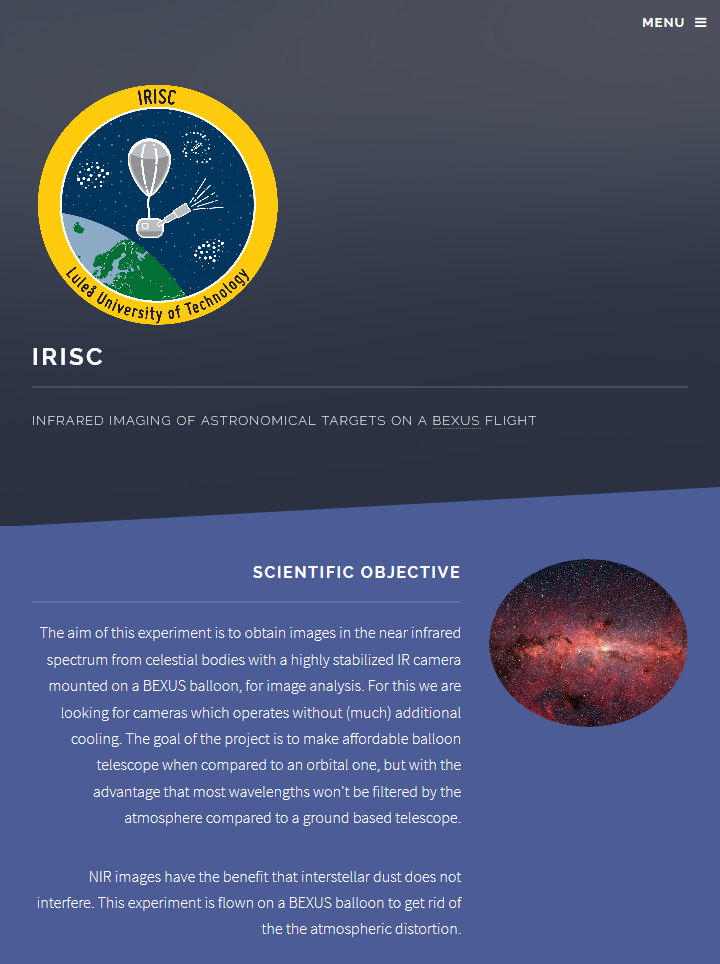
\includegraphics[width=0.9\linewidth]{figures/images/website.png}
    \end{minipage}%
\end{figure}
\end{frame}


%----------------------------------------------------------------------------------------
%	SUMMARY.
%----------------------------------------------------------------------------------------
\section{Summary}
\begin{frame}[t]{Summary} 		% ????
\centering
\begin{itemize}
    \item Proof of concept of a stabilised balloon-borne telescope with an NIR camera
    \item Empowered by the BEXUS project
    \item To achieve a higher degree of accessible and affordable astronomical research
    %\item Outreach to the public by website, social media, presentations, TV \& newspapers.
\end{itemize}

\begin{figure}
    \vspace{-.3cm}
    \subfloat{
        
\includegraphics[height=0.25\textwidth, valign=c]{figures/logos/IRISC_Black.png}
    } \hspace{2cm}
    \subfloat{
        
\includegraphics[height=0.25\textwidth, valign=c]{figures/logos/bexus.png}
    } 
\end{figure}
\end{frame}

\begin{frame}{IRISC}
    \centering
    \Huge Thank you for your attention\\\vspace{.3cm}
    \Large Let us explore the NIR universe with a BEXUS balloon together!\\
    
    %\huge Questions?\\\
    \vspace{1cm}
    \large \insertauthor \\\vspace{.2cm}%\insertauthor \\\vspace{.2cm}
    and the rest of the IRISC team
\end{frame}

%----------------------------------------------------------------------------------------
%	QUESTIONS.
%----------------------------------------------------------------------------------------
\section{Questions}
\begin{frame}{IRISC}
    \label{slide:questions}
    \centering
    \vspace{-0.71cm}
    \begin{figure}
    \hspace*{-1.1cm}
    	\includegraphics[width=1.15\textwidth]{figures/images/teamphoto.png}
    \end{figure}
\end{frame}

%----------------------------------------------------------------------------------------
%	BACKUP SLIDES. 				EVERYONE!!!
%----------------------------------------------------------------------------------------





%----------------------------------------------------------------------------------------
%	BACKUP SLIDES: 		ELECTRICAL
%----------------------------------------------------------------------------------------
\subsection{Electrical}
\begin{frame}[t]{Cooling electrical systems in space}
    The only way to get rid of thermal energy, outside the lower atmosphere, is radiation. Passive solutions are:
    \begin{itemize}
        \item Highly efficient components.
        \item Passive cooler with fluid (convection).
        \item Solid thermal conducting material connected to the heat sources (conduction).
    \end{itemize}
    
        \centering
        \vspace{1cm}
        \begin{figure}
            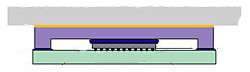
\includegraphics[width=.5\textwidth]{figures/images/Passive_cooler_2.jpg}\\
            \caption{Clemens J. M. Lasance, cooling electronics}
        \end{figure}
\end{frame}

\begin{frame}{Schematic: Sensors \& onboard computer}
	\vspace{-.2cm}
	\begin{figure}
		
\includegraphics[width=.68\textwidth]{figures/schematics/elec01.png}
	\end{figure}
\end{frame}

\begin{frame}{Schematic: Gyroscopes}
	\vspace{-.2cm}
	\begin{figure}
		
\includegraphics[width=.68\textwidth]{figures/schematics/elec02.png}
	\end{figure}
\end{frame}

\begin{frame}{Schematic: Motor Controller}
	\vspace{-.2cm}
	\begin{figure}
		
\includegraphics[width=.68\textwidth]{figures/schematics/elec03.png}
	\end{figure}
\end{frame}

\begin{frame}{Schematic: Thermal Sensors}
	\vspace{-.2cm}
	\begin{figure}
		
\includegraphics[width=.68\textwidth]{figures/schematics/elec04.png}
	\end{figure}
\end{frame}

\begin{frame}{Schematic: Heating System}
	\vspace{-.2cm}
	\begin{figure}
		
\includegraphics[width=.68\textwidth]{figures/schematics/elec05.png}
	\end{figure}
\end{frame}

\begin{frame}{Schematic: Power Management}
	\vspace{-.2cm}
	\begin{figure}
		
\includegraphics[width=.68\textwidth]{figures/schematics/elec06.png}
	\end{figure}
\end{frame}

%------------Control system - Anja-------------%

\subsection{Control System}
\begin{frame}[t]{Control System}
    \vspace{-0.5cm}
    \begin{figure}
        \centering
        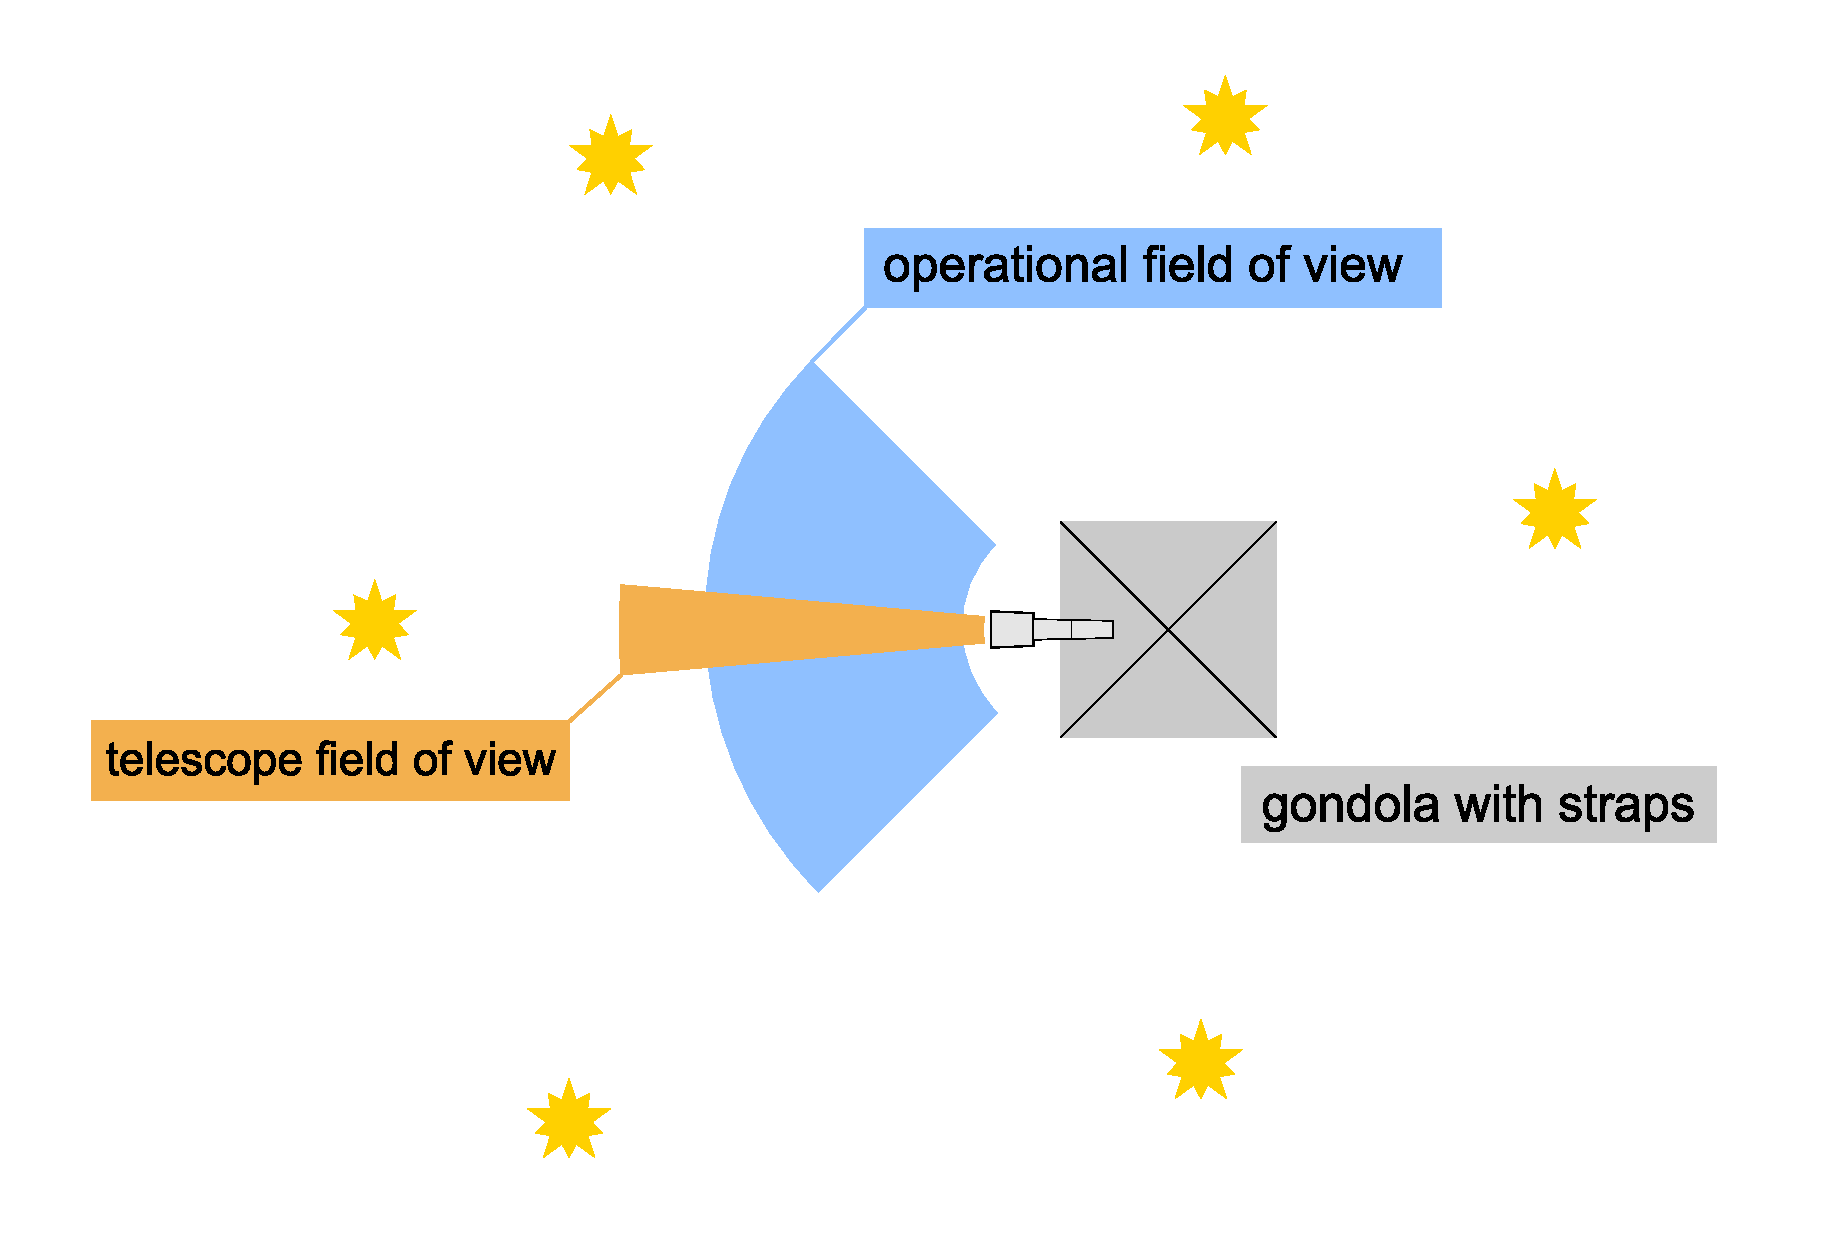
\includegraphics[width=0.7\textwidth]{figures/images/FoV_telescope.eps}
        \label{fig:FoV}
        %\caption*{Credit: https://publiclab.org/wiki/public-lab-lesson-3-photography-in-a-new-light}
    \end{figure}
\end{frame}

%------------Science - Kim --------------%

\subsection{Science}
\begin{frame}[t]{Telescope}
\begin{figure}[!htb]
    \centering
    \begin{minipage}{.5\textwidth}
        \centering
        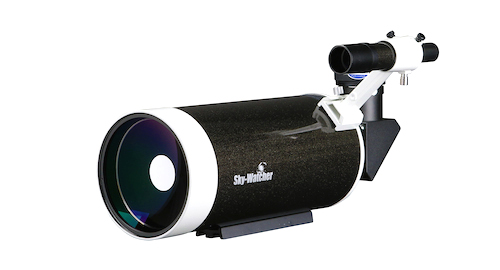
\includegraphics[width=\linewidth]{figures/images/SkyWatcher_BKMAK127OTAW.jpg}
        \caption*{SkyWatcher BK MAK127 OTAW (with eyepiece in place of the camera)}
    \end{minipage}%
    \begin{minipage}{0.5\textwidth}
    SkyWatcher BK MAK127 OTAW
    \begin{itemize}%[label=--]
        \item Cassegrain telescope 
        \item Physical length: 33\,cm
        \item Focal length: 1500\,mm 
        \item Aperture: 127\,mm
        \item FOV: 0.5\,deg by 0.34\,deg 
        \item Diffraction-limited-resolution: 2.01\,arcsec
        \item Pixel size: 0.33\,arcsec (in \newline combination with the camera)
    \end{itemize}
    \end{minipage}
\end{figure}
\end{frame}


\begin{frame}[t]{Targets (brightness-ordered)}
\begin{table}[]
\tiny
\begin{tabular}{|c|c|c|c|c|c|c|}
\hline
\textbf{Name}                  & \textbf{Designation} & \textbf{RA}    & \textbf{DEC}    & \textbf{Mag}  & \textbf{Dim x (arcsec)} & \textbf{Dim y (arcsec)} \\ \hline
Andromeda Galaxy      & M31         & 0.70  & 41.27  & 3.44 & 190   & 60    \\ \hline
Open Star Cluster     & M52         & 23.40 & 61.58  & 5    & 13    & 13    \\ \hline
Reflection Nebula     & NGC 1333    & 3.48  & 31.35  & 5.6  & 6     & 3     \\ \hline
Triangulum galaxy     & M33         & 1.55  & 30.65  & 5.72 & 70.8  & 41.7  \\ \hline
Hercules Globular     & M13         & 16.68 & 36.45  & 5.8  & 20    & 20    \\ \hline
Eagle Nebula          & M16         & 18.30 & -12.18 & 6    & 7     & 7     \\ \hline
Iris Nebula           & NGC 7023    & 21.02 & 68.17  & 6.8  & 18    & 18    \\ \hline
Veil Nebula           & NGC 6992    & 20.75 & 30.70  & 7    & 180   & 180   \\ \hline
The Wizard Nebula     & NGC 7380    & 22.78 & 58.10  & 7.2  & 25    & 25    \\ \hline
Pacman Nebula         & NGC 281     & 0.87  & 56.62  & 7.4  & 20    & 30    \\ \hline
Starfish Open Cluster & M38         & 5.47  & 35.85  & 7.4  & 21    & 21    \\ \hline
Crescent Nebula       & NGC 6888    & 20.20 & 38.35  & 7.4  & 18    & 12    \\ \hline
Dumbbell Nebula       & M27         & 19.98 & 22.72  & 7.5  & 8     & 5.6   \\ \hline
Pinwheel galaxy       & M101        & 14.05 & 54.33  & 7.8  & 28.8  & 26.9  \\ \hline
Whirlpool Galaxy      & M51         & 13.48 & 47.18  & 8.4  & 11.2  & 6.9   \\ \hline
Cigar Galaxy          & M82         & 9.92  & 69.67  & 8.41 & 11.2  & 4.3   \\ \hline
Intergalactic Tramp   & NGC 2419    & 7.63  & 38.87  & 9.06 & 6     & 6     \\ \hline
Sunflower galaxy      & M63         & 13.25 & 42.02  & 9.3  & 12.6  & 7.2   \\ \hline
Bubble Nebula         & NGC 7635    & 23.33 & 61.20  & 10   & 15    & 8     \\ \hline
\end{tabular}
\end{table}
\end{frame}

%------------Budget - Niklas-------------%

\subsection{Budget} 			% NIKLAS
\begin{frame}{Budget}
\begin{figure}[!htb]
	\centering
    \begin{minipage}{0.3\textwidth}
	Secured funding:
	\begin{itemize}
		\item LTU Project funds
	\end{itemize}
	Potential funding:
	\begin{itemize}
		\item SNSA
		\item Trusts and foundations
		\item Crowdfunding
		\item Sponsorships
	\end{itemize}
	\end{minipage}%
	\begin{minipage}{0.7\textwidth}
	\centering
	\begin{table}[h]
		\begin{tabular}{|c|c|}
		\hline
		\textbf{Category} & \textbf{Total Price [EUR]} \\ 	\hline
		Structure & 1000 \\ \hline
		Electronics Box & 1000 \\ \hline
		Telescope & 1500 \\ \hline
		Cables and Sensors  &  \\ \hline
		Tools & TBD \\ \hline
		Travel & TBD \\ \hline
		Contingency & TBD  \\ \hline
		{\textbf{Total without Error Margin}} & \textbf{TBD} \\ \hline
		Shipping Costs and Error Margin  &  \\ \hline
		{\textbf{Total with Error Margin}} & \textbf{TBD} \\ \hline
		\end{tabular}
	\end{table}
	
	\end{minipage}
\end{figure}
\end{frame}

\end{document}
